\documentclass{ppig}
\usepackage{epsfig}
\usepackage{booktabs}
\usepackage{ucs}
\usepackage[utf8x]{inputenc}

% The titlebox defines how much vertical space is given for
% the authors' list. If you need extra space to show all the
% authors, uncomment the line below and increase the value. Please
% do not make the titlebox smaller than the original size of 5cm.
%\setlength\titlebox{5cm}

\title{PPIG Papers: Author Instructions and Template File}

% List the authors like you would in a table.
% The \And command creates another author's column. Use it after the
% details of one author to separate them from the following author horizontally.
% The \AND command creates a new "row" of authors and it should be used
% when the authors don't fit on the same line. You may have to increase
% the titlebox so that the author's don't overlap with the abstract.
\author{Alan F. Blackwell \\
  Computer Laboratory \\
  University of Cambridge \\
  Alan.Blackwell@cl.cam.ac.uk \\
  \And
  Luke Church \\
  Computer Laboratory \\
  University of Cambridge \\
  luke@church.name \\
  \And
  Mariana M\unichar{259}r\unichar{259}\unichar{537}oiu\\
  Computer Laboratory \\
  University of Cambridge \\
  mcm79@cl.cam.ac.uk}

\date{}

\begin{document}
\maketitle
\thispagestyle{empty}

\begin{abstract}
This file both describes and exemplifies the required format for papers submitted to PPIG 2016. Please review this file even if you have submitted to PPIG before as some formatting details have changed relative to previous years.
\end{abstract}

\section{Introduction}

This format is to be used for all PPIG 2016 paper submissions for review and camera-ready versions. The easiest way to do this is to replace the current content of this file with your own material.

The rest of this document describes the format you should use when preparing your submission.

\section{Formatting instructions}

\subsection{Page size}

The paper should be A4 (21 $\times$ 29.7 cm or 8.27 $\times$ 11.69 inches). The margins around the text should be of 1 inch (2.54 cm) each and the text should be justified, not left-aligned/ragged. The length of the paper should not exceed the maximum 12 page limit. Pages should not be numbered.

\subsection{Fonts}

The fonts used in this paper are Times Roman or Times New Roman, Arial or Helvetica for headings and Courier for source code. Table~\ref{tbl:font-guide} summarises the font sizes and styles used for each part of this file. For Microsoft Word users, the default styles have been replaced to follow the settings here. For \LaTeX{} users, the \texttt{ppig.cls} applies the settings described here to your \texttt{.tex} file.

\begin{table}[h]
	\begin{center}
		\begin{tabular}{@{}cccc@{}}\toprule
			Type of text & Font & Font size & Style\\\midrule
			Paper title & Arial/Helvetica & 12pt & Bold\\
			Author names & Times Roman & 11pt & Bold\\
			Author affiliations & Times Roman & 11pt &\\
			The word "abstract" & Arial/Helvetica & 11pt & Bold\\
			Abstract text & Times Roman & 11pt &\\
			Section level 1 & Arial/Helvetica & 11pt & Bold\\
			Section level 2 & Arial/Helvetica & 11pt &\\
			Document text & Times Roman & 11pt & \\
			Caption & Times Roman & 11pt & Italic\\
			Code & Courier & 11pt &\\
			Bibliography & Times Roman & 11pt &\\
			Footnotes & Times Roman & 10pt &\\
			\bottomrule
		\end{tabular}
		\caption{Font guide.}
		\label{tbl:font-guide}
	\end{center}
\end{table}


\subsection{Title and authors}

The title, author's name(s) and affiliation(s) should be centred at the top of the first page. The title should be in Arial or Helvetica 12pt bold font. The author's name(s) should be in Times New Roman or Times Roman 11pt bold font, and their affiliation(s) should be in Times New Roman or Times Roman 11pt font.

The author's name(s) and affiliation(s) is created using a table with invisible borders and one row in Microsoft Word and a table with no borders and a row for each line in \LaTeX. In order to add a new author in Microsoft Word, add a new column to the table and enter the author's details. For \LaTeX users, please follow the instructions in the \texttt{ppig-submission-template.tex} file.

If all authors have the same affiliation, you may choose to have a single affiliation block, with author's name(s) and email address(es) separated by commas. To do so, use a single column table.

\subsection{References}

The references section at the end of this template shows the style that should be used for references. The references themselves should preferably follow the format of the APA (American Psychological Association) style guide, although we won't be too strict about the details. Citations should be in APA format: \citeA{blackwell1999how} says the year should be in parentheses after mention of the author's name. In cases where the author's name is not in the sentence, the citation gives name and year in parentheses \cite{blackwell1999how}.

\subsection{Figures and Tables}

Tables and Figures should fit within the boundaries of the text on this template file, and should be centred on the page. Both figures and tables can be placed inline with the text (e.g. Fig.~\ref{fig:sample-figure}), but the text shouldn't wrap around their sides. Use your own judgement to create suitable tables and figures. Figures and tables should have captions. Captions for both figures and tables should use the caption style defined in Table~\ref{tbl:font-guide}.

\begin{figure}[h]
	\centering
	\epsfig{file=sample-figure.eps, scale=0.5}
	\caption{A sample figure, with caption}
	\label{fig:sample-figure}
\end{figure}

\section{Submission Procedure}

Submissions must be in PDF format.

TBD

\section{Acknowledgements}
Thank you to Mariana M\unichar{259}r\unichar{259}\unichar{537}oiu for updating this template for PPIG 2016, to Luke Church and Alan Blackwell for defining this template and to Eleonora Bilotta, Thomas Green and Paola Kathuria for their help in defining and testing this template.

\bibliography{ppig-sample-bibliography}
\bibliographystyle{apacite} 
\end{document}
